\chapter{Destructive 3D phenotyping pipeline}

\section{Introduction}

Estimating the plant phenotypes accurately and efficiently can help to bridge the gap between genotype and phenotype. The traditional phenotyping measurement is time-consuming, laborious, and often not accurate. Although several authors have developed 2D image-based phenotyping methods which are more efficient, non-destructive, and have higher throughput \citep{yang_greenness_2015,guo_easypcc_2017,zou_broccoli_2019}, these approaches are unable to describe the plant 3D structure due to the occlusion and dimension loss when projecting onto the 2D plane. As a result, it produces inaccuracies and uncertainties for advanced phenotyping applications.

To overcome the drawbacks of 2D image-based phenotyping, several studies have paid attention to 3D approaches. \citet{paulus_measuring_2019} and \citet{kochi_introduction_2021} have summarized the current approaches to obtain 3D plant models; and a large number of studies have chosen the 3D reconstruction by photogrammetry using common RGB cameras due to the low device cost \citep{xiao_estimating_2021,zermas_3d_2020,zhang_estimating_2016}. The 3D model of an object can be calculated from images from different view angles with enough overlap (Fig.~\ref{fig:des1}). The full process includes structure-from-motion (SfM, to calculate relative positions between images and the rough 3D point cloud of the object), multi-view stereo (MVS, to densify the 3D point cloud of the object), and surface reconstruction (to obtain object 3D mesh model); for more details, please refer to this book \citep{hartley_multiple_2000} and this review \citep{snavely_scene_2010}. Although the proposed 3D image-based phenotyping was proved feasible for many agriculture applications, when apply to the broccoli head cases, the current 3D method is facing several challenges.

\begin{figure}[htb]
  \begin{center}
    \resizebox{\textwidth}{!}{
      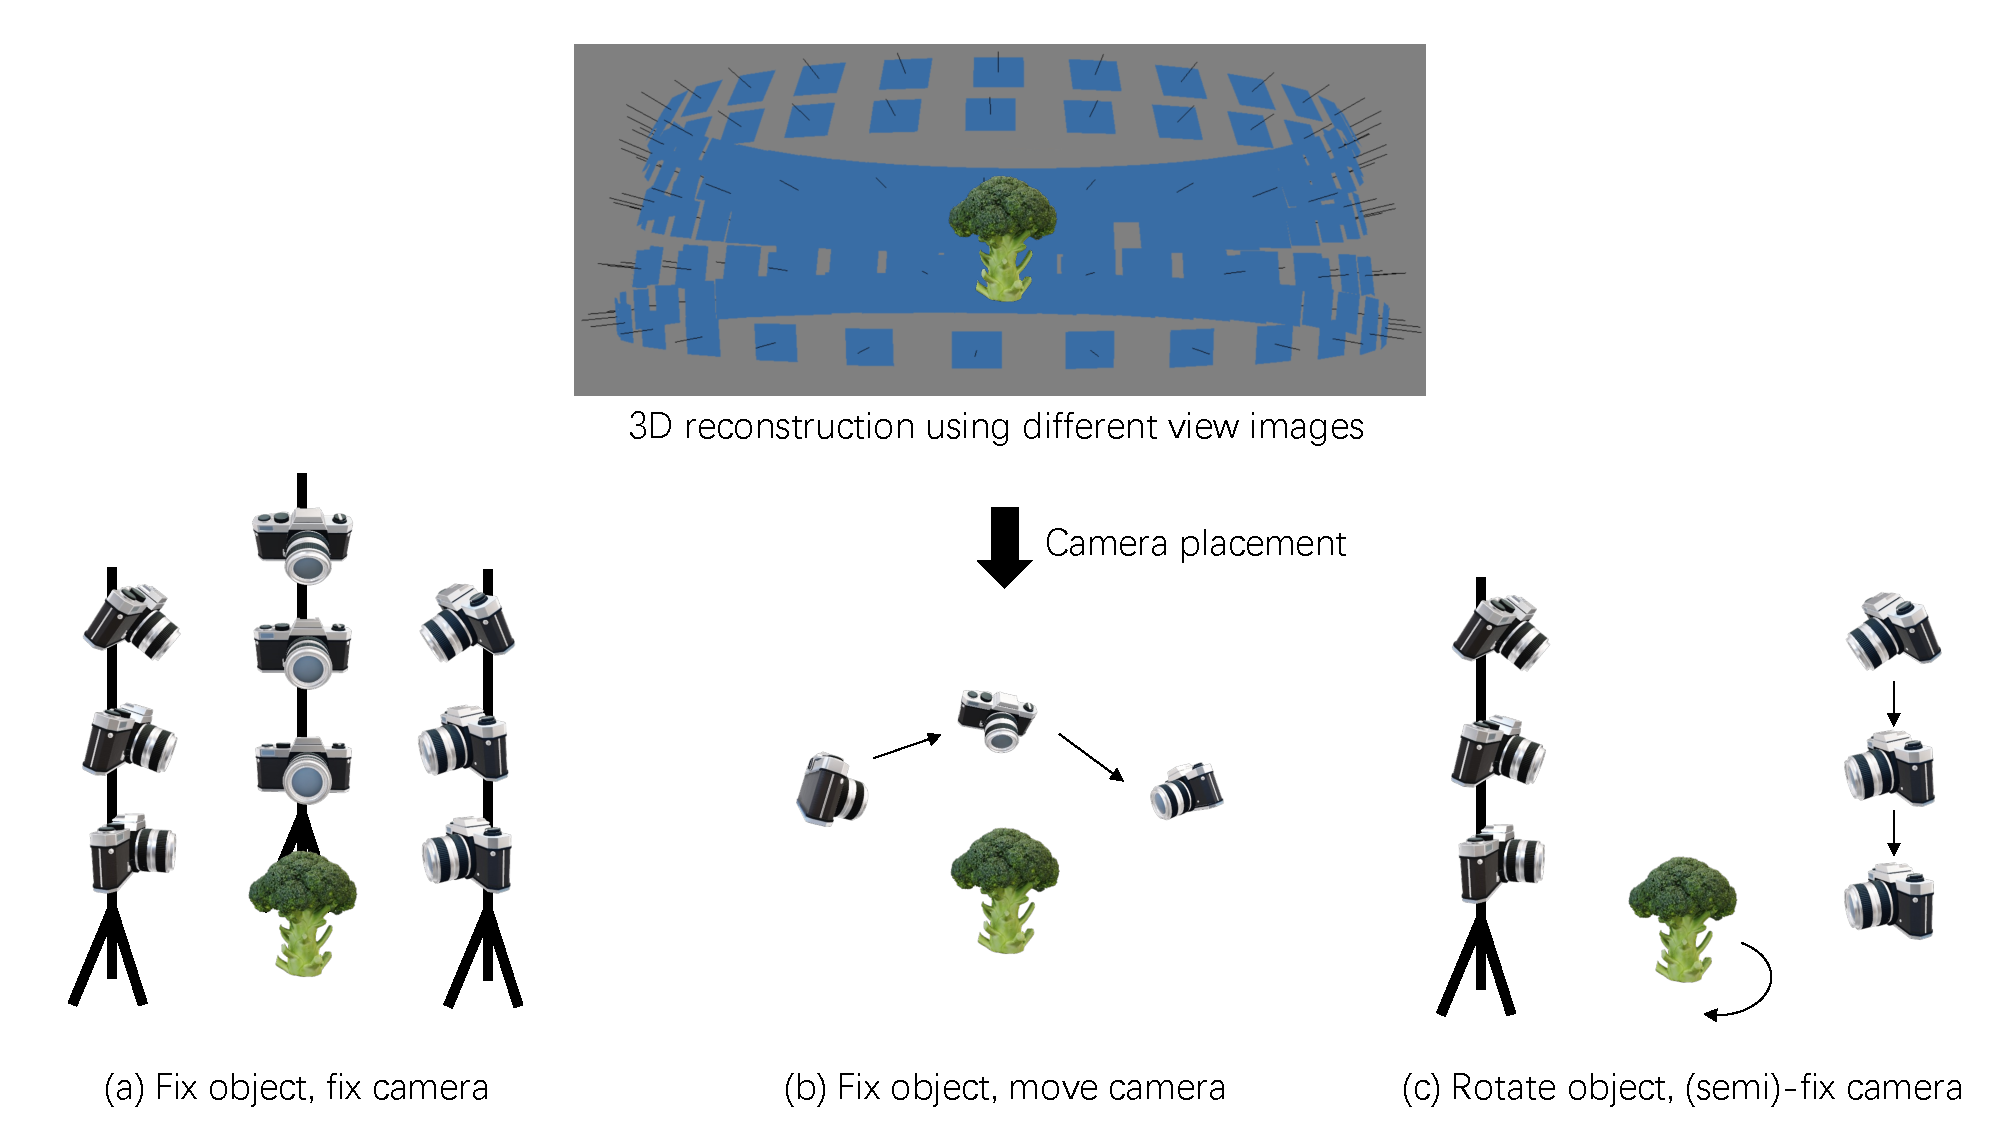
\includegraphics{figures/des/sfm_types.pdf}
    }
  \end{center}
  \caption[Current photogrammetry (3D reconstruction) methods and challenges]{
    The current photogrammetry (3D reconstruction) methods and challenges; (a-c) the current image acquisition approaches (a) fixing the object and taking images using multiple fixed cameras at the same time, also called forward intersection; (b) fixing the object but taking images by using a moved camera, also called backward resection; and (c) rotating the object and taking images using fewer multiple fixed cameras, or a camera fixed at different locations for each rotation. The challenges of current approaches: (d) the limited view angles of current image occlusion approaches has visual dead area, which will cause incomplete plant 3D models; and (e) the difficulties to segment foreground (plant) area in the image preprocessing.
  }
  \label{fig:des1}
\end{figure}

The first challenge is image acquisition for cost-effective reconstruction. Several authors used the following three approaches to acquire images (Fig.~\ref{fig:des1}): (a) fix the object and fix cameras \citep{nguyen_structured_2015}; (b) fix the object and move a camera manually \citep{xiao_image-based_2020} or using robotic arms \citep{cao_quantifying_2019,nguyen_3d_2016}; and (c) rotate the object and fix or move the camera(s) \citep{kochi_3d_2018,gao_novel_2021}. The main drawback of these imaging approaches is that it is difficult to provide fully complete view angles of plants within acceptable cost. Most methods can only capture images of the sunny side (such as the front surface of leaves and the top of broccoli crowns); while capturing images of the shaded side (such as the back surface of leaves and the downside of broccoli crowns) is more difficult and requires extreme upward viewing angles (Fig.~\ref{fig:des1}d). Even if such images can be acquired, they often fail to align with the 3D model due to insufficient feature matching points. Hence, a solution is required to improve the integrity of the reconstructed plant 3D model, especially for the solid closed harvestable organs like broccoli heads.

The second challenge is image preprocessing for the acquired images. Compared to the approach of building the full scenario, segmenting the plant parts out \citep{ge_method_2019}, and denoising \citep{wu_mvs-pheno_2020}; some studies segmented and masked the foreground (plant) area before doing the 3D reconstruction \citep{nguyen_3d_2016,kochi_3d_2018}, to improve the model quality and eliminate the effect of background noises. Although the controlled environment can provide pure background and stable lighting, it is still challenging to develop a robust algorithm to segment the broccoli area perfectly, especially to handle the shadows caused by the irregular broccoli head shape at the different growing stages. Some outdoor studies showed the power of deep learning for plant area detection and segmentation \citep{zhou_monitoring_2020,blok_effect_2021,garcia_towards_2021}, but limited by the GPU memory, the original images often resized to smaller sizes for deep learning. For example, \citet{zhou_monitoring_2020} resized to $1440 \times 1080$, \citet{blok_effect_2021} resized to $1024 \times 1024$, and \citet{garcia_towards_2021} resized to $640 \times 480$. The plant mask produced in such a resolution can not fit well into the original images in detail (in our case, is $5184 \times 3456$), and hence also need a method to produce detailed masks with the original resolution.

In this study, we applied several strategies to overcome the previously mentioned challenges and provide a labor-saving pipeline for obtaining high-quality 3D models for destructive broccoli heads. The objectives of this study were to (1) develop the dual-rotation object strategy with a fixed camera to collect images with abundant view angles for integrity 3D reconstruction; (2) implement the two-step deep learning workflow to acquire the detailed plant masks on the original images; (3) calculate the 3D morphological traits of broccoli head and crown; and (4) validate the estimated head size using the manual measurements. This pipeline also has great potential to be applied to other solid closed harvestable organs, such as potatoes, cauliflowers, and sweet potatoes, which are related to the profit directly. Meanwhile, using just a simple RGB camera and several low-cost commercial photographic equipment, makes it easier to be widely-spread use.


\section{Methods and Materials}

The pipeline proposed in this study has two main parts, the workflow to acquire high-quality broccoli head 3D models and the workflow to measure the morphological traits of broccoli heads. For the first workflow, we developed an automatic imaging device using commercial photographic equipment, which extended the design of \citet{kochi_3d_2018} to dual-rotation of objects; then applied marker detection (software built-in function) and deep learning segmentation of plant masks to the collected images, as image preprocessing; afterward, we extended our previous batch scripts in the \citet{feldman_easydcp_2021} to automatically operate the 3D reconstruction on a large number of broccoli heads to get 3D model results. For the second workflow, similar to our previous work \citep{feldman_easydcp_2021}, we first developed the unsupervised algorithm to split broccoli crown and stem parts; then corrected the broccoli head top direction of the 3D models (as the z-axis positive direction); lastly, we calculated several 2D and 3D morphological traits of the broccoli head and segmented crown.

\subsection{Plant materials}

Field trials were conducted at the experimental farm of the Institute for Sustainable Agro-ecosystem Services (ISAS), Nishi-Tokyo, Tokyo, Japan ($35^\circ 43'$N, $139^\circ 32'$E) from October 2021 to April 2022. The plot sizes were approximately $3000 m^2$; The meteorological data during the growth period were collected by a local weather station and are shown in Table~\ref{tbl:des1}. The soil was tilled and leveled using Half-Soiler and a Rotary implement. Then, the initial fertilizer was mechanically spread and mixed thoroughly on 11 October 2021; around 11,000 broccolis (cultivar: suzuka[すずか]) were machine transplanted with a plant spacing of $35 cm$ and row spacing of $70 cm$ was done from October 14 to 16; and additional fertilizer was applied by hand on October 28. Herbicides, insecticides, and fungicides were applied as needed using mechanical spreaders.

\begin{table}[htb]
  \caption{Meteorological data during the experiment period}
  \label{tbl:des1}
  % \begin{adjustwidth}{-0.05\textwidth}{-0.05\textwidth}
    \begin{center}
      \resizebox{1\textwidth}{!}{
        \begin{tabular}{cccc}
          \hline
                  & \begin{tabular}[c]{@{}c@{}}Mean temperature\\ ($^\circ C$)\end{tabular} & \begin{tabular}[c]{@{}c@{}}Total precipitation\\ ($mm$)\end{tabular} & \begin{tabular}[c]{@{}c@{}}Mean daily solar radiation\\ ($MJ \cdot m^{-2}$)\end{tabular} \\ \hline
          2021.10 & 17.6                                                                    & 156.5                                                                & 11.2                                                                                     \\
          2021.11 & 12.2                                                                    & 85.0                                                                 & 11.0                                                                                     \\
          2012.12 & 6.4                                                                     & 123.0                                                                & 9.6                                                                                      \\
          2022.01 & 3.6                                                                     & 16.5                                                                 & 10.6                                                                                     \\
          2022.02 & 3.8                                                                     & 60.0                                                                 & 13.3                                                                                     \\
          2022.03 & 10.3                                                                    & 94.5                                                                 & 15.3                                                                                     \\
          2022.04 & 15.0                                                                    & 213.0                                                                & 15.9                                                                                     \\ \hline
        \end{tabular}
      }
    \end{center}
  % \end{adjustwidth}
\end{table}

Three fertilizing treatments (inorganic, organic, and mixed) with three replicates (total 9 plots) were applied to examine their effects on broccoli heads in another study \citep{nishida_estimation_2023}. In this study, We randomly destructively sampled the same number of continuous broccolis for each plot during the growing seasons for indoor 3D reconstruction. 

\subsection{Plant 3D model acquisition}

The general workflow to acquire a broccoli head 3D model is shown in Figure~\ref{fig:des_img_recons}, including imaging devices, image pre-processing, and batch reconstruction.

\begin{figure}[htb]
  \begin{center}
    \resizebox{\textwidth}{!}{
      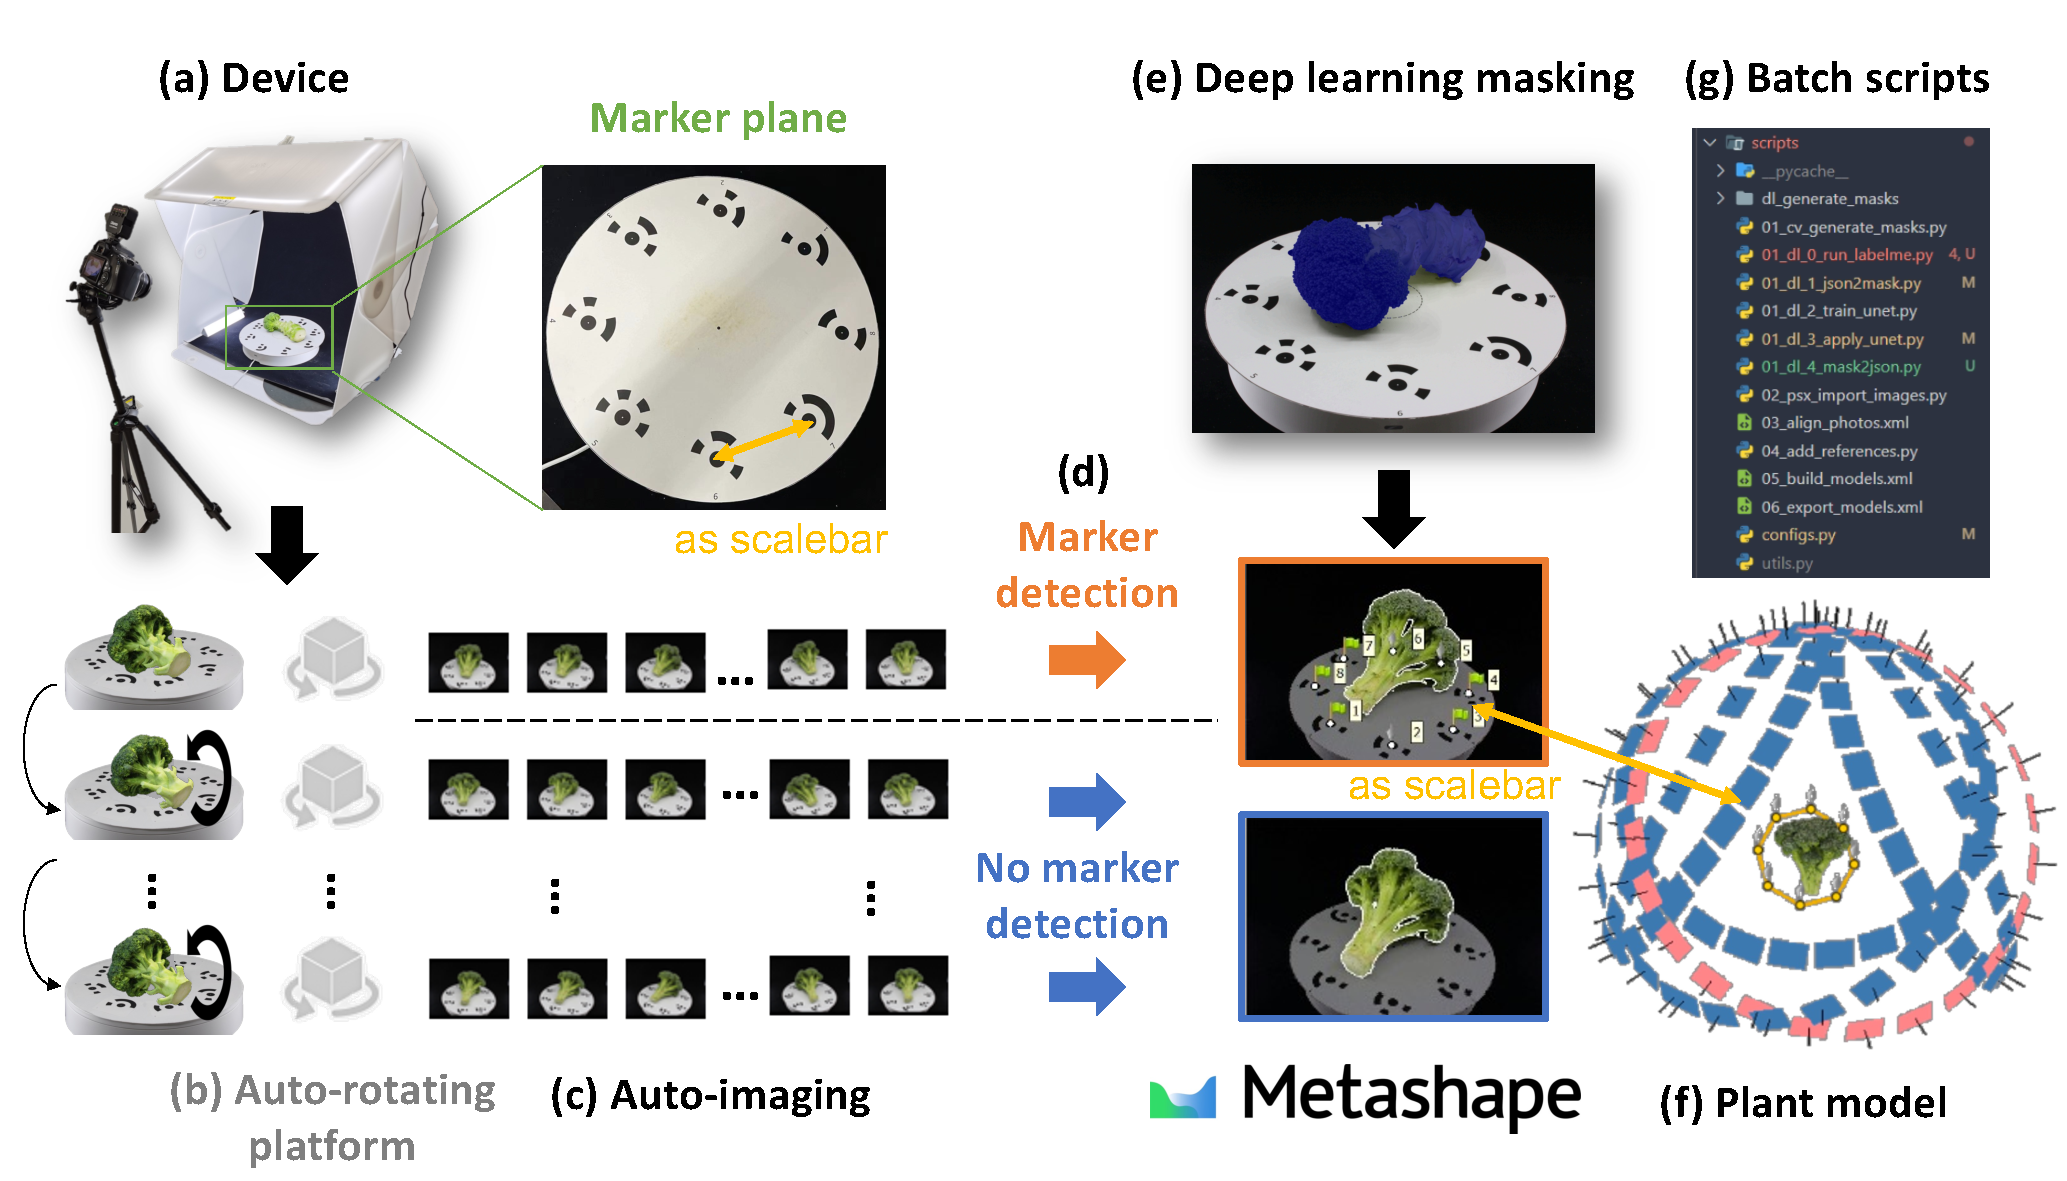
\includegraphics{figures/des/img_recons.pdf}
    }
  \end{center}
  \caption[The plant 3D model reconstruction workflow]{
    The Plant 3D model reconstruction workflow; (a) devices for taking plant images, with a marker plane used as scalebar references; (b) an automatic horizontal rotating platform, which can rotate at a given angle and then stop for a short interval for image taking. The vertical rotation of plants (flip) requires manual operation; (c) different photographic perspectives images taken by the infrared signal auto-imaging system; (d) partial marker detection to avoid misleading image alignment, where only markers on one rotating image group (orange) are detected and not on the others (blue); (e) plant part segmentation using deep learning; (f) the final 3D plant model produced by Metashape; and (g) the scripts for batch processing a large number of plants.
  }
  \label{fig:des_img_recons}
\end{figure}

The imaging device is assembled by a marker board, an automatic horizontal rotating platform (Foidio360, \url{https://orangemonkie.com/ja/products/foldio360-turntable}), a small photography studio (with lighting and pure color background), a Canon EOS 60D digital single-lens reflex (DSLR) camera, and a tripod (Fig.~\ref{fig:des_img_recons}a). The rotating platform can rotate at a given angle ($15^\circ$ in this study) and then stop for a short interval for image taking. It can emit infrared to control DSLR cameras to take photos and directly transfer images to a computer through a data cable and Canon EOS Utility 2 software (\url{https://cweb.canon.jp/drv-upd/dc/euw21401.html}, Fig.~\ref{fig:des_img_recons}c). But manually rotating the broccoli head vertically (black rotation arrow in Fig.~\ref{fig:des_img_recons}b) around three to five iterations are required to get enough view angles for complete 3D reconstruction. The commercial software, Agisoft Metashape (\url{https://www.agisoft.com}), is used to conduct the 3D reconstruction.

The 3D reconstruction and the later image and data processing are conducted on a computer with an AMD Ryzon 9 5950x with 16-Core processors, the RAM is DDR4 128GB. The computer also has one Nvidia GeForce RTX 3090 graphical processing unit (GPU). The operating system is Windows 11 Professional. The codes are implemented in Python 3.8, CUDA 11.1, Pytorch 1.8.2, and torchversion 0.9.2. For more package requirements.

The first image preprocessing is partial marker detection (Fig.~\ref{fig:des_img_recons}d). The marker board not only provides reference points for camera alignment but also provides the size calibration as a scalebar. The Metashape provides the built-in function to detect markers on the given images. However, only markers on the first rotating image group (orange color) are detected and not on the others (blue color). It is because we vertically rotate the plants, the relationship between the plant and markers changes and can mislead the expected image alignment from other rotation groups. In other words, the position relationship between the camera and the marker board does not change after the vertical rotation of the broccoli head, but we want to ``cheat'' the software by that it is the camera movement around the broccoli head (Fig.~\ref{fig:des_img_recons}f). This also requires masking off those background areas in the images.

We use two pre-trained deep-learning networks for the second image processing of plant area segmentation (masking). As mentioned in the introduction, deep learning can handle complicated image analyzing tasks, but often not fits with the original image resolution. Here we first use a pre-trained UNet with default model setting (\url{https://github.com/qubvel/segmentation_models.pytorch}) and do the transfer training with only 19 broccoli images. The training data is annotated using the open-source software, Labelme (\url{https://github.com/wkentaro/labelme}). The UNet model produces rough masks ($256 \times 256$ pixel resolution) with good performance and acceptable processing speed on almost all broccoli head images during the growing season. Afterward, we directly use the pre-trained CascadePSP \citep[\url{https://github.com/hkchengrex/CascadePSP}]{cheng_cascadepsp_2020} to refine the rough masks to the original image resolution without any image annotation (Fig.~\ref{fig:des_img_recons}e). Afterward, to further address the potential flaws of the previous segmentation results, we assume the plant area should be one continuous region. Hence, we only keep the largest region as the plant area and fill the small holes inside the plant area, as the final result.

And finally, we develop the batch scripts for the previous image preprocessing and the 3D reconstruction control in the Metashape (Fig.~\ref{fig:des_img_recons}g). The scripts and detailed use instructions can be found at \url{https://github.com/UTokyo-FieldPhenomics-Lab/Foldio360_3D_Reconstruct_Platform}.

\subsection{Morphological traits extraction}

The workflow of Morphological traits extraction is shown in Figure~\ref{fig:des_seg_alg}, which includes broccoli crown segmentation, direction correction, and traits calculation.

\begin{figure}[htbp!]
  \begin{center}
    \resizebox{0.9\textwidth}{!}{
      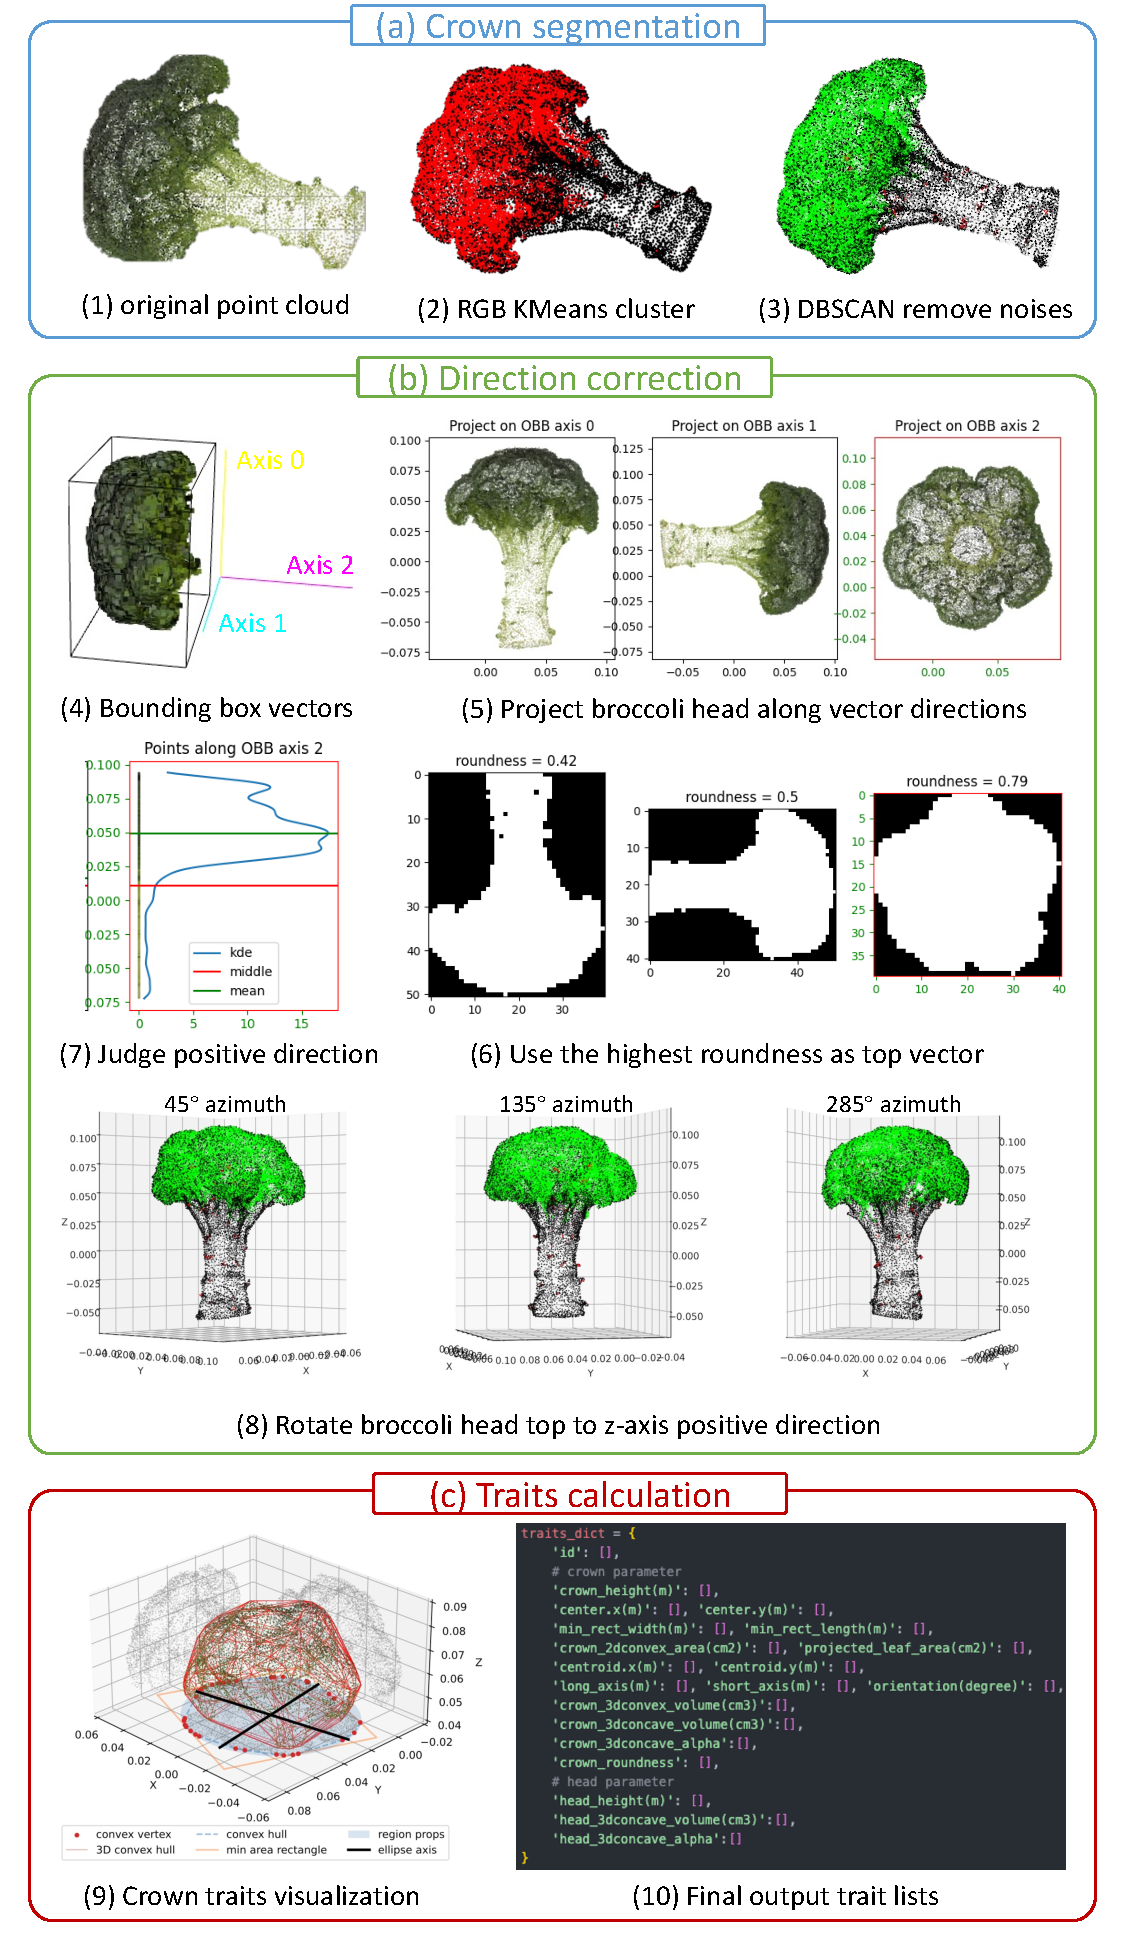
\includegraphics{figures/des/seg_algorithm.pdf}
    }
  \end{center}
  \caption[The algorithms for plant 3D model analysis]{
    The algorithms for plant 3D model analysis; (a) crown segmentation, to split the broccoli crown part and the stem part; (b) direction correction, to rotate the broccoli vertically to the z-axis positive direction; and (c) traits calculation.
  }
  \label{fig:des_seg_alg}
\end{figure}

The broccoli crown segmentation part aims to split the crown and the stem. Since they have significant color differences, the color information can be used for splitting. But simply using a color threshold, e.g. \citet{otsu_threshold_1979} threshold, does not work in our pre-experiment, because the color also variates among individual heads during the growing season. To begin, We first transfer the head 3D mesh models to a point cloud with RGB colors (Fig.~\ref{fig:des_seg_alg}a1). Then use the unsupervised Kmeans clustering algorithm to split all point clouds into two classes (Fig.~\ref{fig:des_seg_alg}a2). Later, the mean RGB color values of these two classes is calculated and transformed into HSV color space. The V represents the ``darkness'' of color, and the class with lower V values (darker color) is picked as the crown part. And finally, we use the DBSCAN algorithm to cluster the crown points into several groups according to neighbor point density. These groups are clustered by 2-class Kmeans again according to their size, the clusters with smaller means sizes are discarded as noises (red dots in Fig.~\ref{fig:des_seg_alg}a3).

Due to the broccoli heads always laying on the marker board (the X-Y plane in the coordinates), the broccoli head top is not following the z-axis positive direction for the reconstructed 3D model. To better find the projecting plane for the crown projecting area and the crown thickness calculation, we need to correct the head top direction. To begin, we calculate the minimum volume bounding box (oriented bounding box, OBB) and the vectors of its three perpendicular edges (Fig.~\ref{fig:des_seg_alg}b4). And the broccoli head has variate shapes during the growing season, the shortest perpendicular edge is not always the top direction. Hence, we project the full broccoli into the corresponding planes perpendicular to OBB vectors (Fig.~\ref{fig:des_seg_alg}b5); and calculate the roundness of the projected shape. The vector with the highest roundness is used as the top direction vector (red boundary, Fig.~\ref{fig:des_seg_alg}b6). Later on, to find out the positive direction (Axis 2 in Fig.~\ref{fig:des_seg_alg}b4 is a reversed direction), we project full broccoli along the vector (left greenish vertical line in Fig.~\ref{fig:des_seg_alg}b7) and calculated the middle value and the mean value of these points. The positive direction should be the middle value greater than the mean value. The figure~\ref{fig:des_seg_alg}b8 shows the corrected direction along the previous vector, with azimuth angle views at $45^\circ$, $165^\circ$, and $285^\circ$.

In the end, similar to our previous work \citep{feldman_easydcp_2021}, we calculate the traits for the broccoli crown (Fig.~\ref{fig:des_seg_alg}c9) and the whole broccoli. For the 1D traits, we calculate the crown height (thickness) and whole broccoli height; For the 2D traits, we project the broccoli crown on the X-Y plane and calculate its center, centroid, roundness, minimum area rectangle width and length, projected area, convex hull area, and the short and long axis and azimuth angle of the fitted ellipse. For the 3D traits, we calculated the 3D convex hull volume for both the crown and whole broccoli and the 3D concave hull volume for the crown only (Fig.~\ref{fig:des_seg_alg}c10).

\subsection{Validation}

To further validate the workflow calculated traits with manually measured traits, considering the difficulty of measuring 2D and 3D traits in reality, here we compared the size of broccoli head only. In agriculture practices, the head lengths are manually measured in the $0^\circ$, $45^\circ$, $90^\circ$, and $135^\circ$ directions (``union jack'') for validation. And then picking the longest and shortest ones as the final size. In the workflow calculated traits, the width and length of the minimum area rectangle, and the long and short axis of the fitted ellipse, have similar definitions for head size descriptions. The agreement of workflow measured and manually measured is estimated using the coefficient of determination ($r^2$, calculated as the squared Pearson's correlation coefficient) and the root mean square error (RMSE):

\begin{equation}
  RMSE = \sqrt{\frac{1}{n} \cdot \sum_{i}^{n} (L_{i}^{W} - L_{i}^{M})^2}
\end{equation}

\noindent
where, $n$ is the total destructive sampled head number, $L_{i}^{W}$ is the  \textbf{W}orkflow calculated length of broccoli head $i$, $L_{i}^{M}$ is the \textbf{M}anually measured length of broccoli head $i$.

\section{Results}

Following the workflow outlined above, we successfully 3D reconstruct a total of 189 destructively sampled broccoli heads during the growing season with high model quality and integrity. The intermediate results also show the feasibility of the proposed algorithms for variate broccoli head shapes. And the calculated traits also have high correlations with manual measurements.

\subsection{Plant 3D model acquisition}

Figure~\ref{fig:des_dl_seg} shows some intermediate results for the plant area segmentation with variate broccoli head sizes and shapes. Using pre-trained UNet and transfer training with just 19 broccoli head images, we generate the rough masks (red parts in Fig.~\ref{fig:des_dl_seg}b) successfully for different broccoli shapes. But limited by the low resolution and a few training data, the UNet does not produce perfect masks, especially on the boundary. Then, the masks are significantly optimized by CasadePSP and the hole-filling postprocessing (blue parts in Fig.~\ref{fig:des_dl_seg}c).

\begin{figure}[htb]
  \begin{center}
    \resizebox{\textwidth}{!}{
      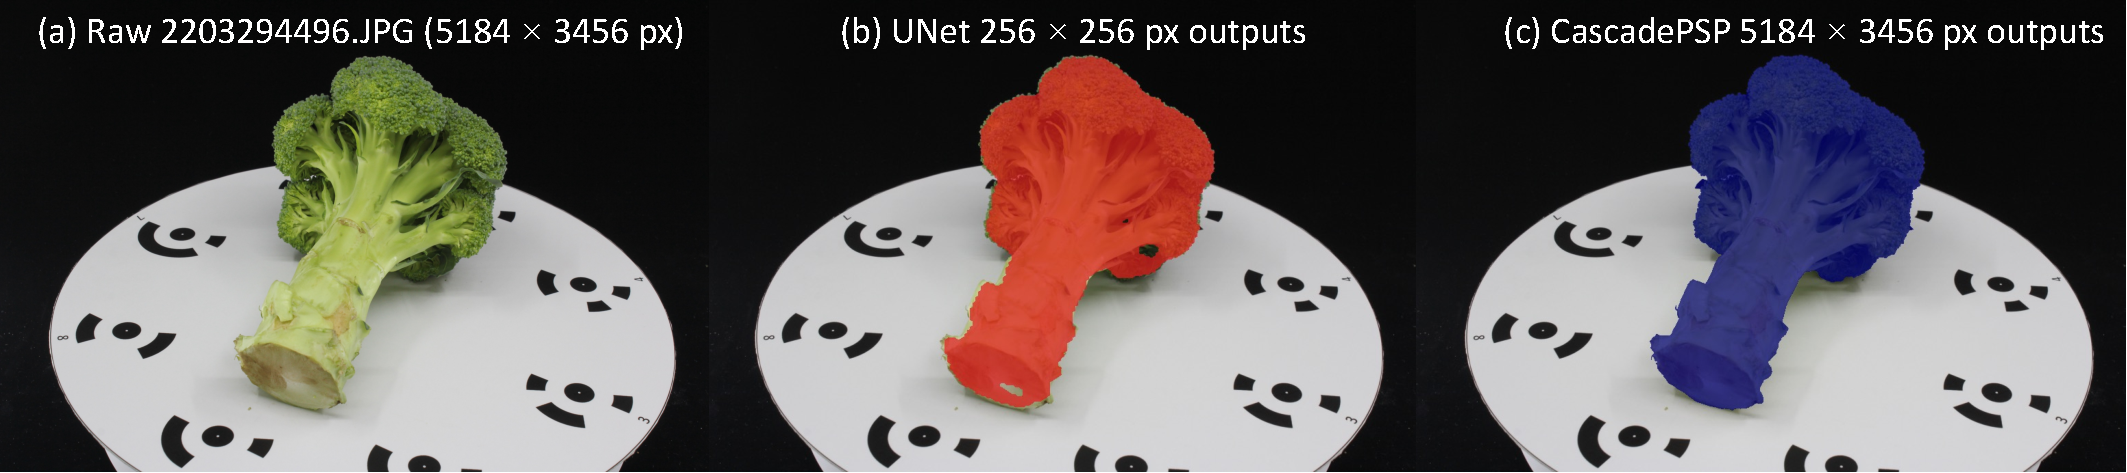
\includegraphics{figures/des/dl_seg.pdf}
    }
  \end{center}
  \caption[Two deep learning segmentation results]{
    An example of two deep learning segmentation results. (a) is the original image of broccoli head id ``2-11'' of rotating group 3, the resolution is $5184 \times 3456$ pixel; (b) is the output of the UNet segmentation, the resolution is $256 \times 256$ pixel, which is not enough as final plant masks; and (c) the output of the refined high-resolution mask using CasadePSP based on the UNet output. The mask has the same resolution as the original image.
  }
  \label{fig:des4}
\end{figure}

Some examples of reconstructed 3D head models are shown in Figure~\ref{fig:des_model_results}. Here we generate a CG image using the 3D head models (Fig.~\ref{fig:des_model_results}b) and compare it visually to the real-world photo (Fig.~\ref{fig:des_model_results}a). Due to limitations in shooting angles and manual editing, the two images are not the same in detail, but the overall details and sizes of the broccoli are quite similar. Figure~\ref{fig:des_model_results}c shows different view angles of the same broccoli head. Unlike other studies whose model bottom \citep{kochi_3d_2018} or leaf backside \citep{cao_quantifying_2019} are not available and may result in the broccoli head crown bottom missing. In general, our proposed dual-rotation workflow produces completely enclosed high-quality 3D models, it will not only contribute to better analysis accuracy but also build a base for future digital farm applications.

\begin{figure}[htb!]
  \begin{center}
    \resizebox{\textwidth}{!}{
      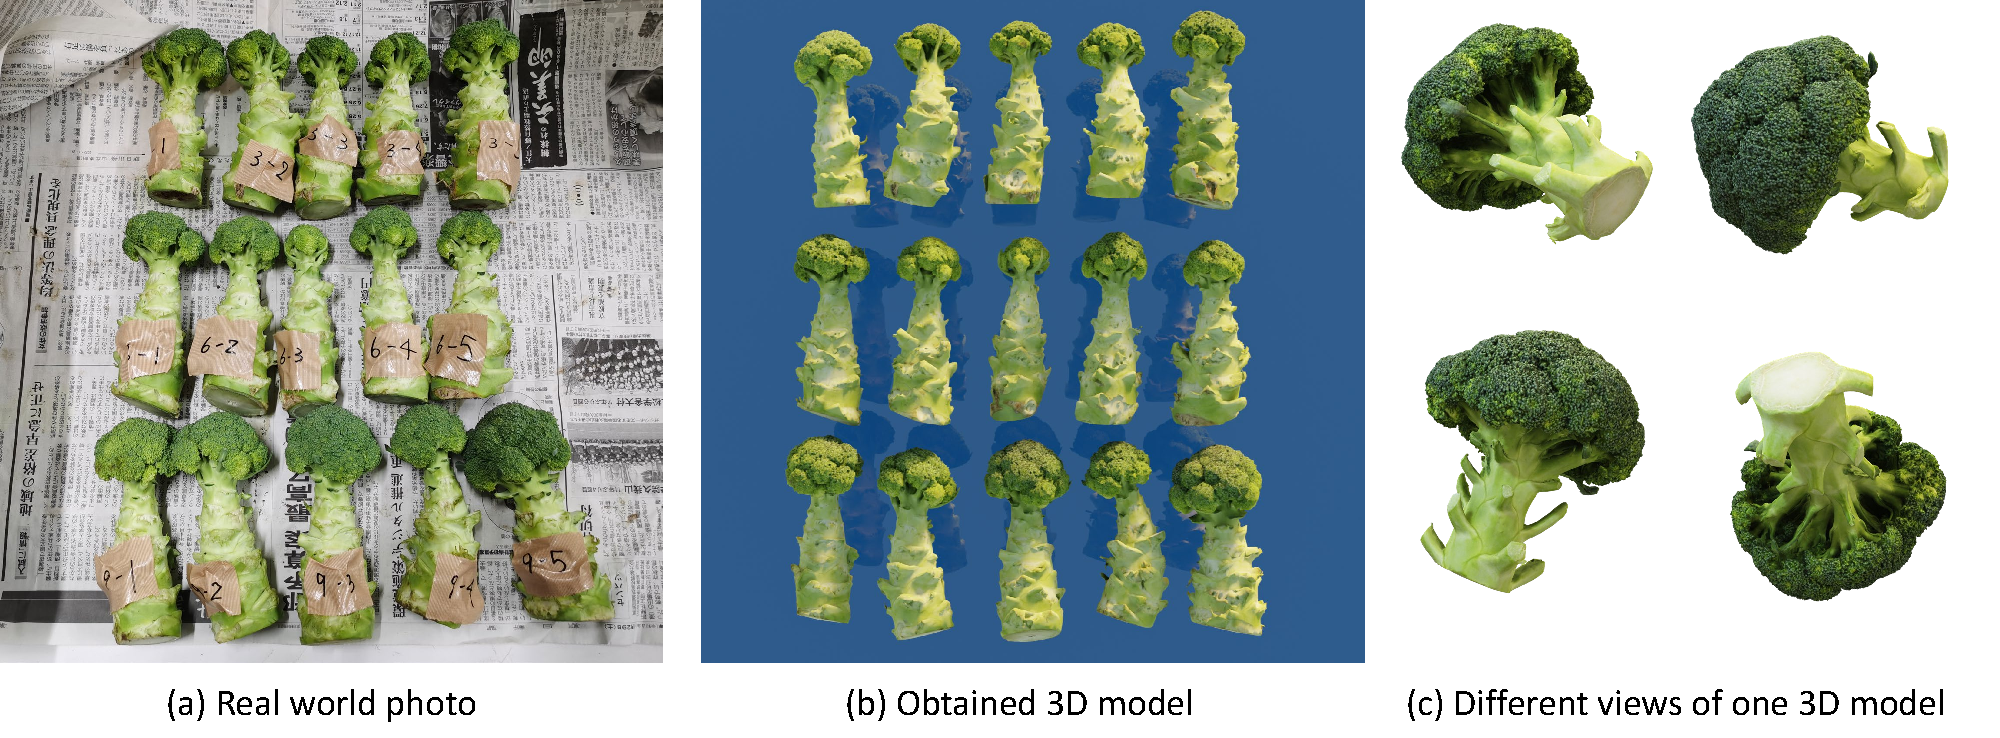
\includegraphics{figures/des/model_results.pdf}
    }
  \end{center}
  \caption[The obtained 3D models]{
    Some examples of obtained 3D models; (a) the image of 15 broccoli heads in the real world; (b) the obtained 3D models of corresponding broccoli heads; and (c) the different views of one broccoli head 3D model.
  }
  \label{fig:des_model_results}
\end{figure}

\subsection{Morphological traits extraction}

As mentioned before, the crown and stem parts of the broccoli head should be segmented and rotated upwards for easier trait calculation. Figure~\ref{fig:des_segrot} shows the feasibility of our proposed unsupervised algorithm on broccoli heads with different shapes. Figure~\ref{fig:des_segrot}a is a simple case of a small broccoli head with a straight stem; Figure~\ref{fig:des_segrot}b is a challenging case with a curved stem;  Figure~\ref{fig:des_segrot}c and d are challenging cases for head and stem segmentation. Instead of concluding that our algorithm rotates them to the exact status in the field correctly, it rotates them to a proper horizontal angle with the largest projection area on the X-Y plane and the shortest thickness on the Z-axis. This provides an initialized starting point for later trait calculation, especially very important for the 1D (on the Z-axis) traits and the 2D traits (on the X-Y plane).

\begin{figure*}[htb]
  \centering
  \begin{subfigure}[b]{0.475\textwidth}
    \centering
    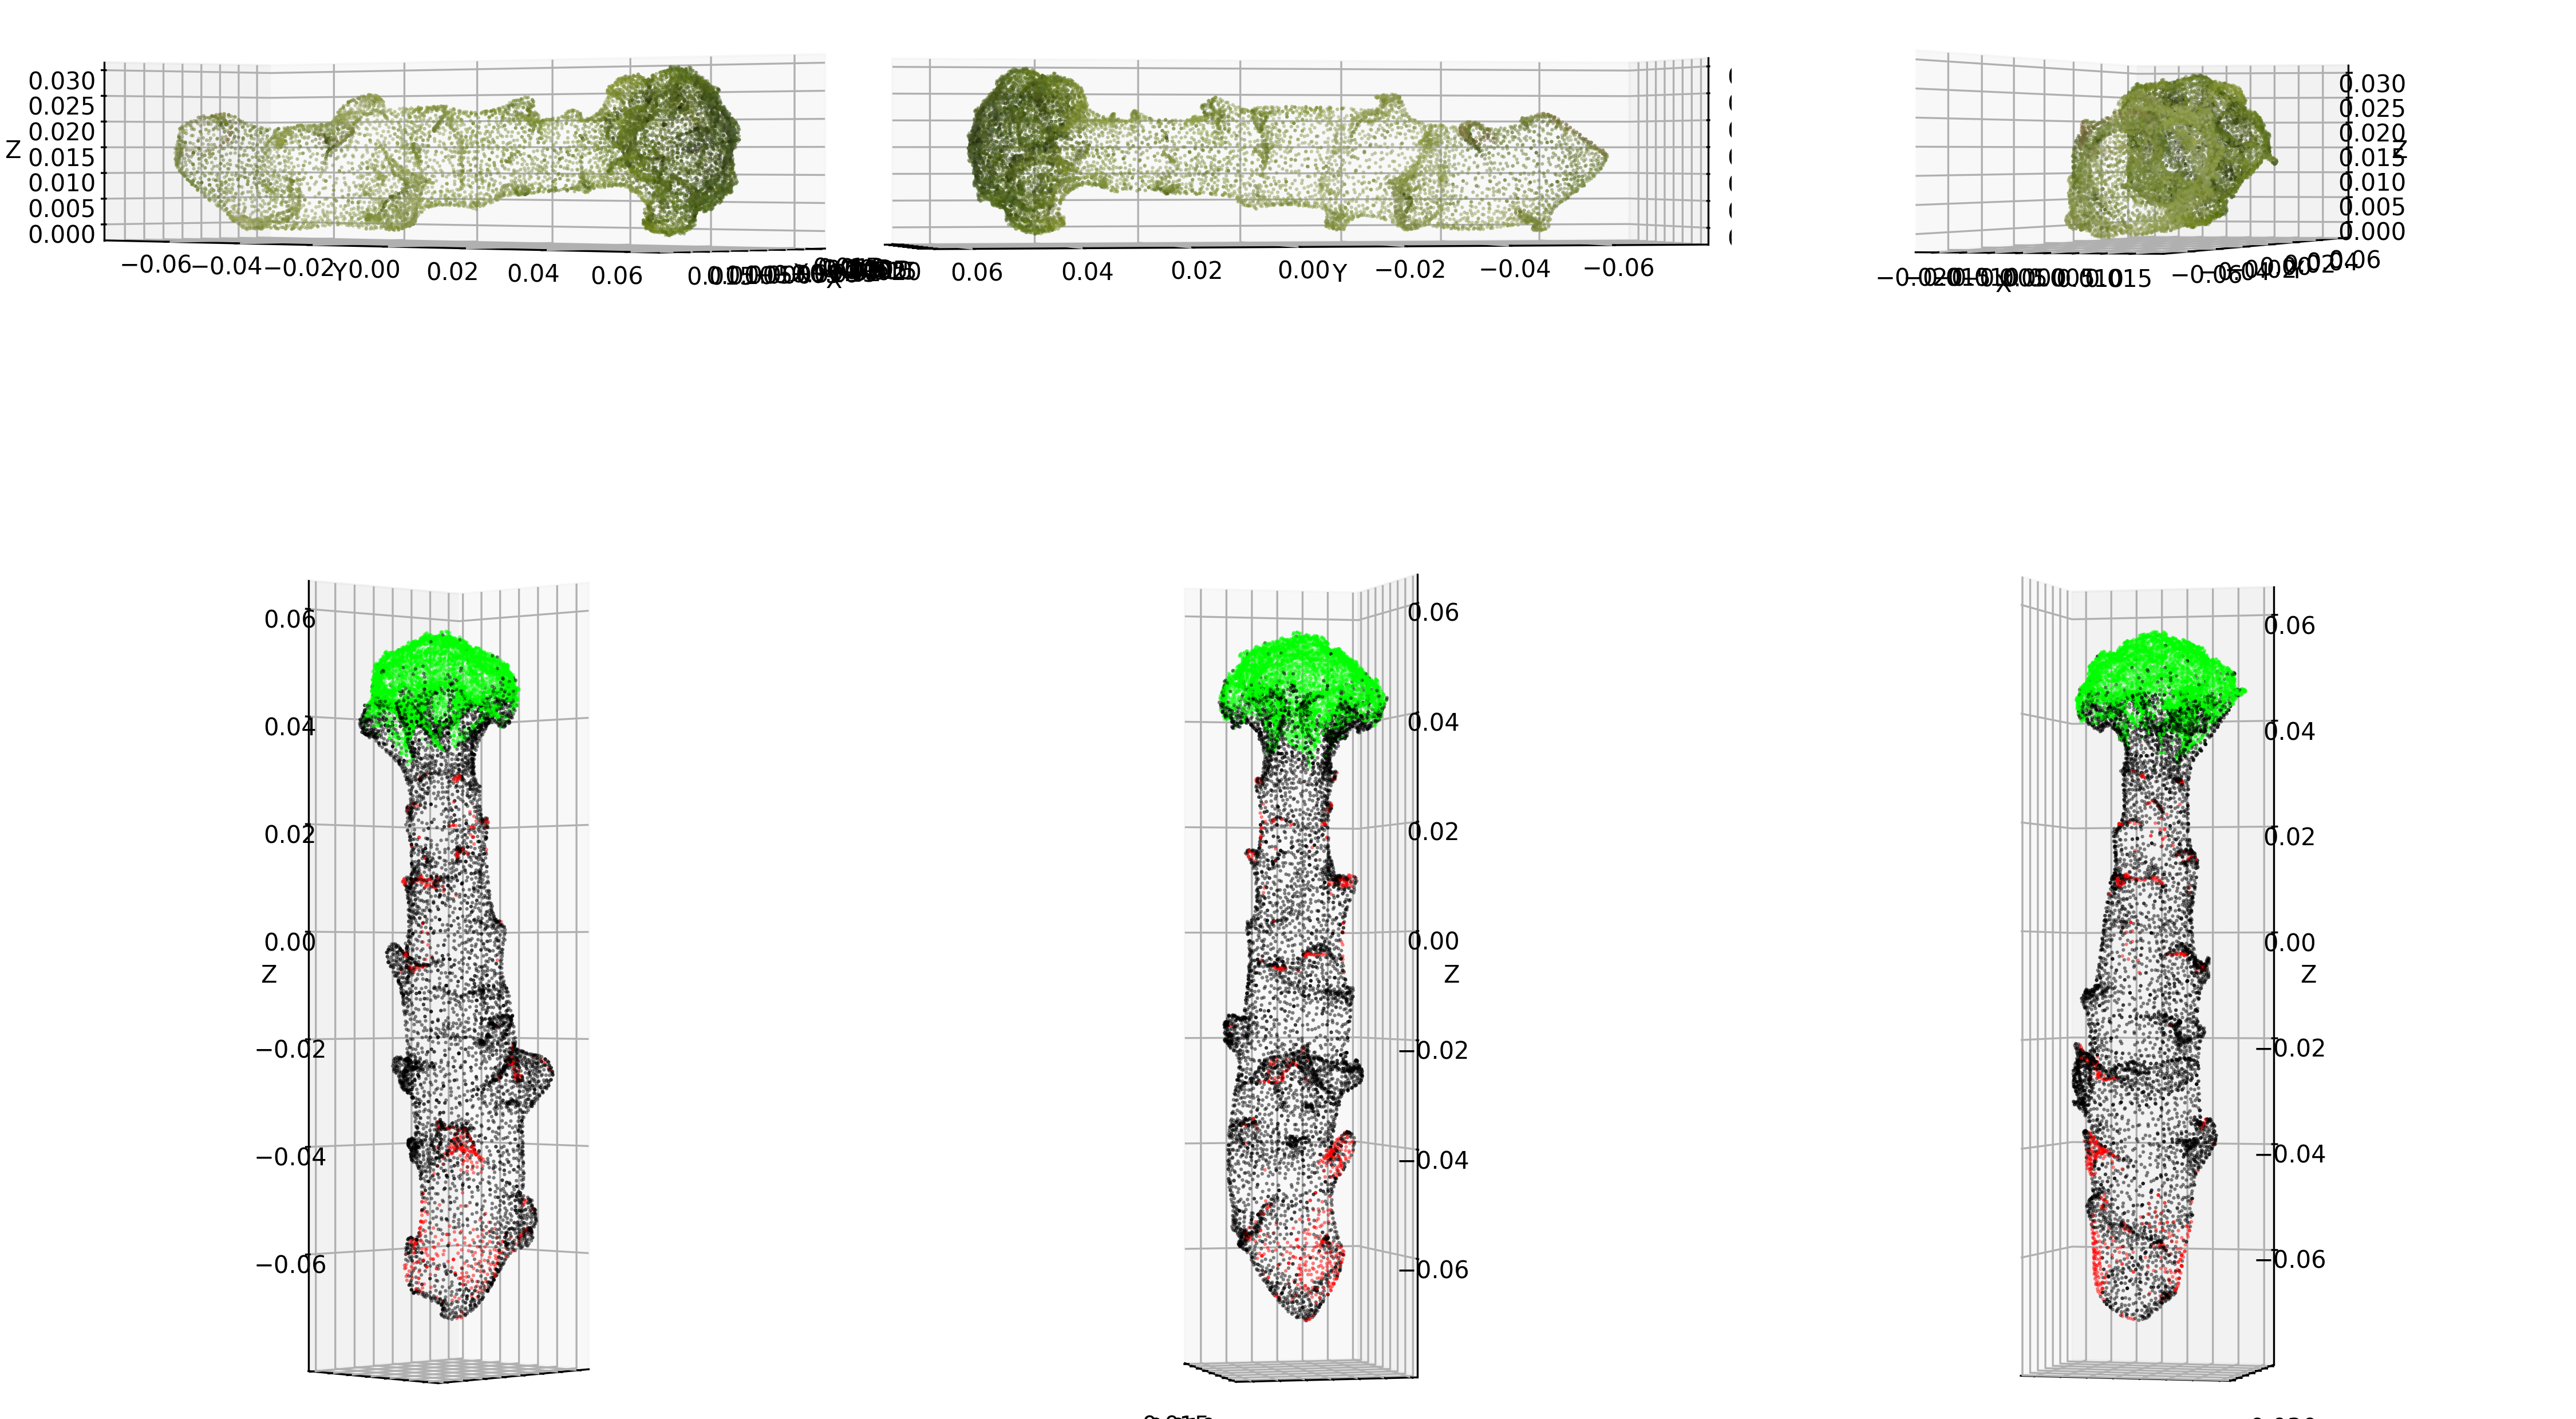
\includegraphics[width=\textwidth]{figures/des/7-2-2.png}
    \caption{ID 7-2-2}
  \end{subfigure}%
  \hfill
  \begin{subfigure}[b]{0.475\textwidth}
    \centering
    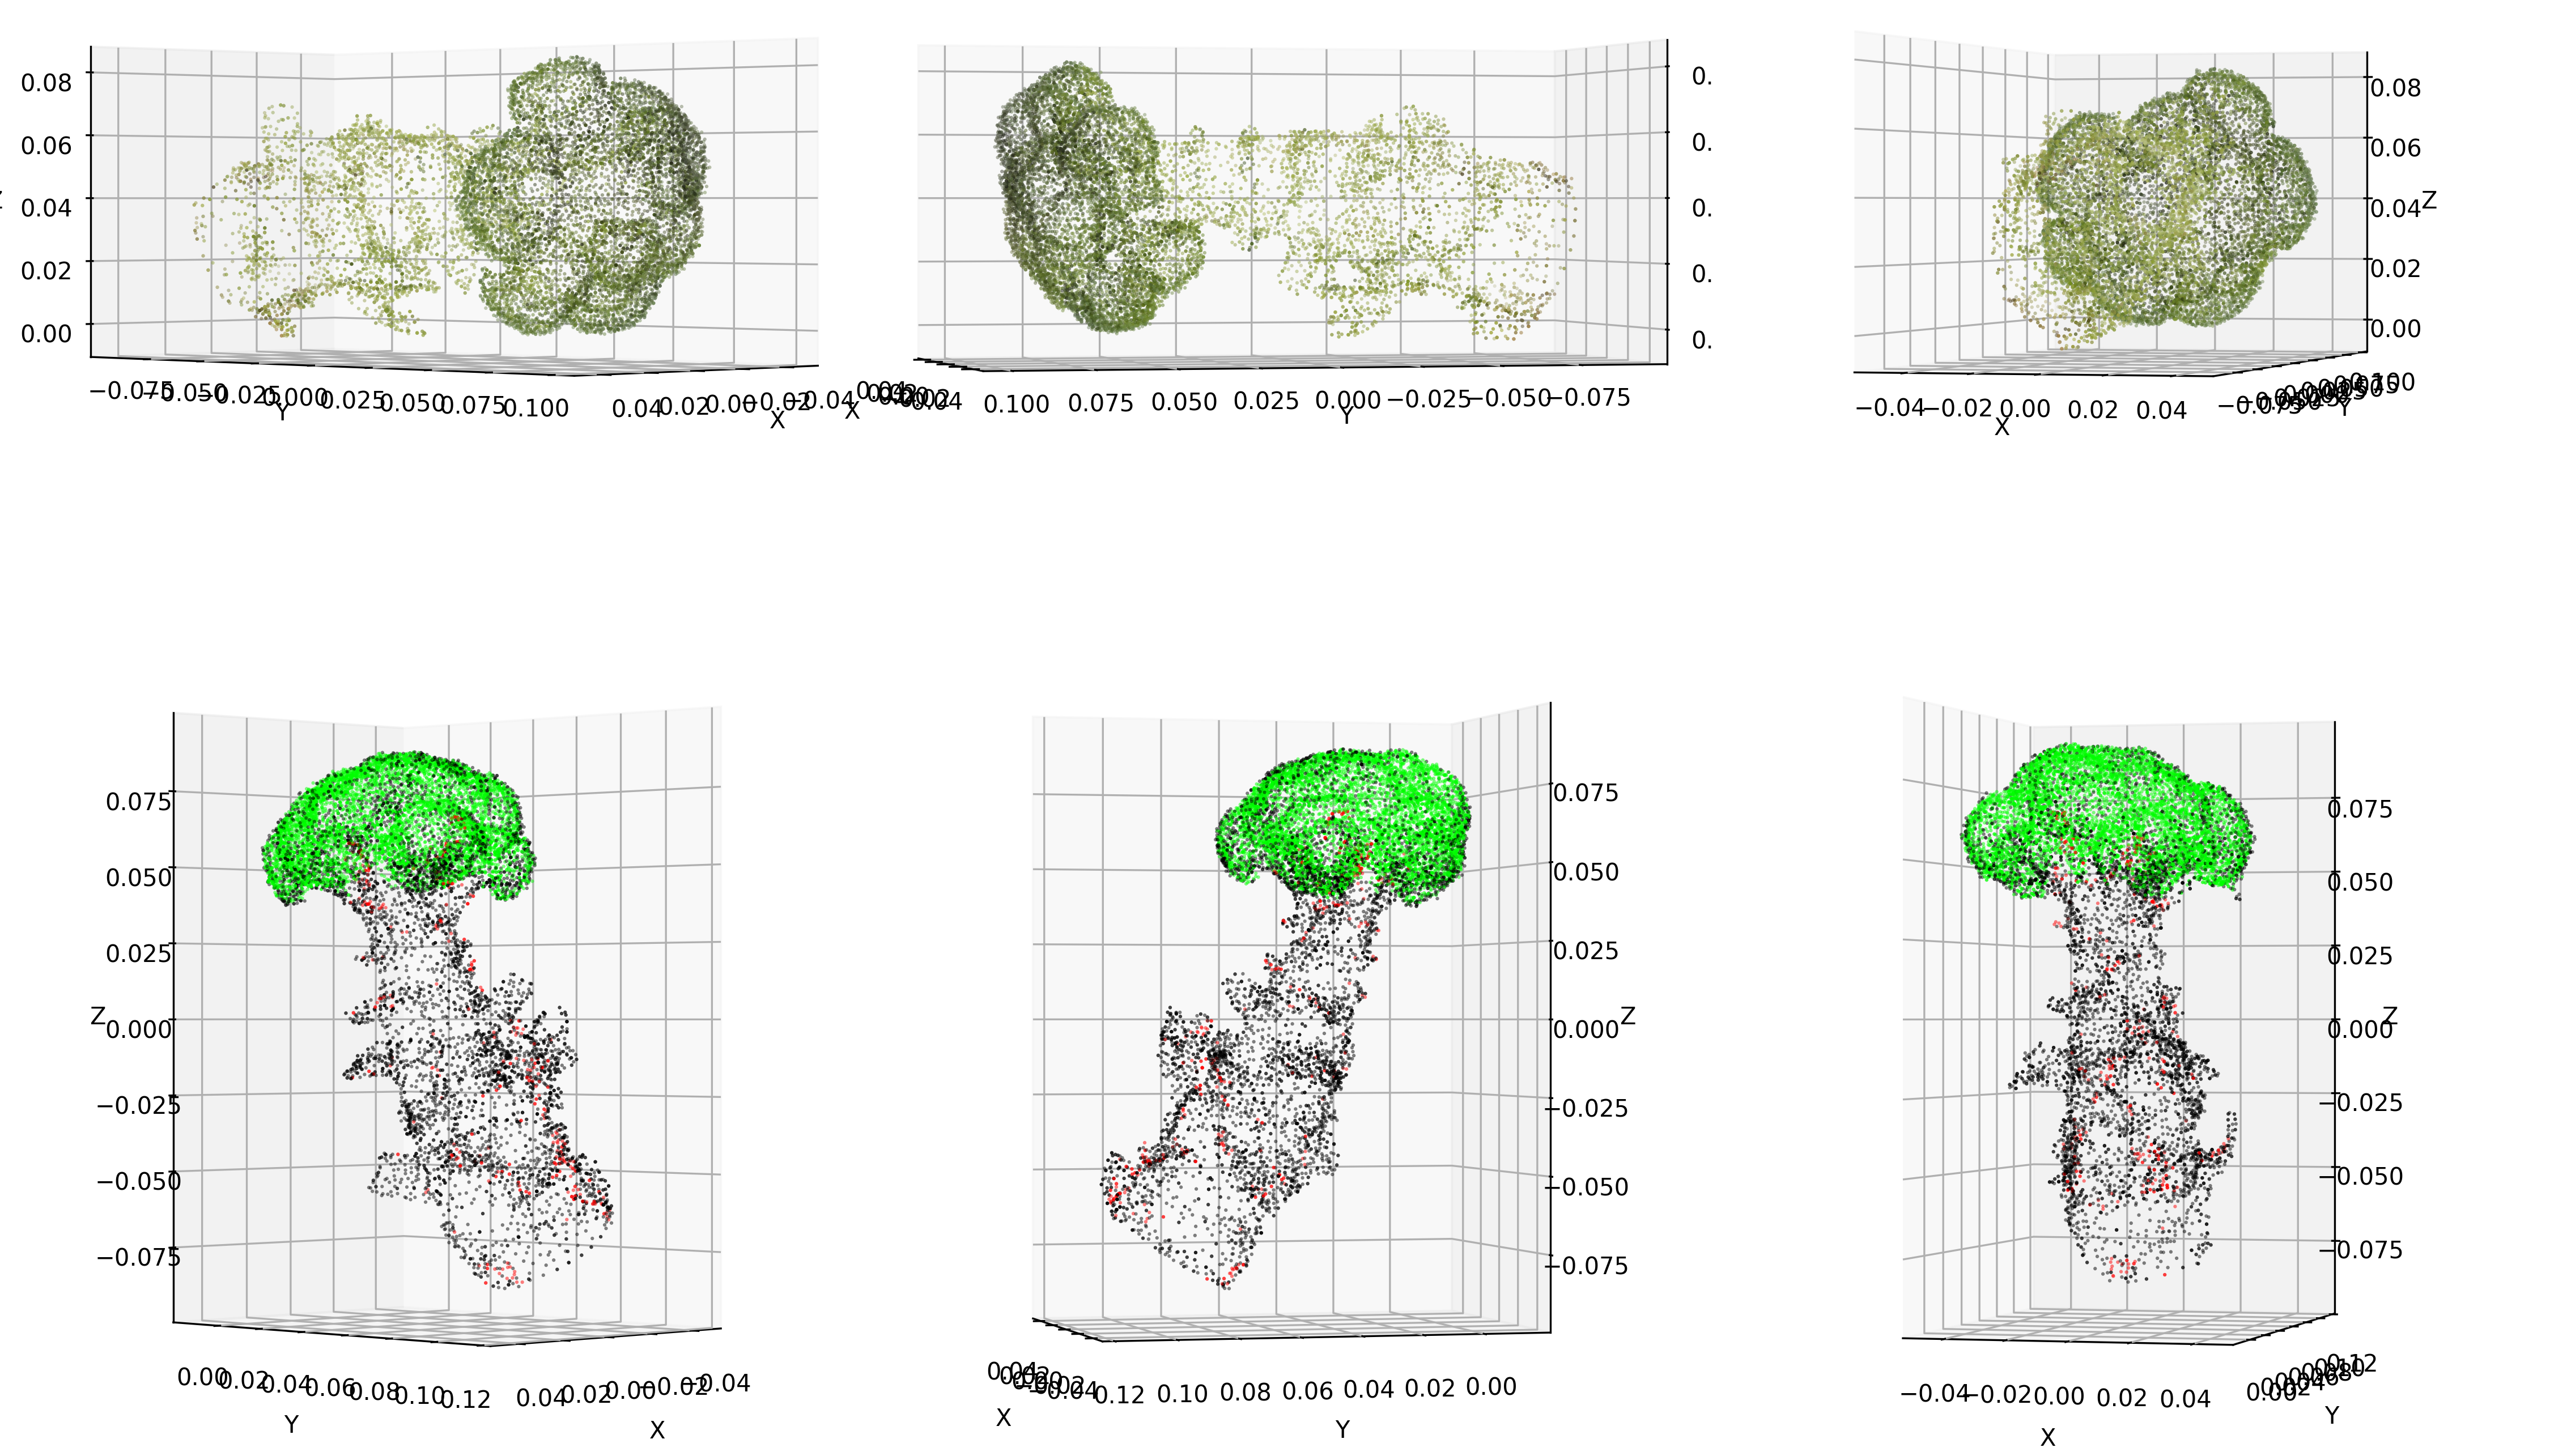
\includegraphics[width=\textwidth]{figures/des/1-5.png}
    \caption{ID 1-5}
  \end{subfigure}
  \vskip\baselineskip

  \begin{subfigure}[b]{0.475\textwidth}
    \centering
    \includegraphics[width=\textwidth]{figures/des/2-23.png}
    \caption{ID 2-23}
  \end{subfigure}%
  \hfill
  \begin{subfigure}[b]{0.475\textwidth}
    \centering
    \includegraphics[width=\textwidth]{figures/des/1-33.png}
    \caption{ID 1-33}
  \end{subfigure}%
  \caption[Examples of plant 3D model analysis at different growing stages]{
    Examples of plant 3D model analysis at different growing stages. The upper parts are the original coordinates of the obtained 3D models, while the lower parts are the segmented and direction-corrected results, the red parts are removed noises. Three columns show the corresponding azimuth angle views at $45^\circ$, $165^\circ$, and $285^\circ$ for the same 3D model.
  }
  \label{fig:des6}
\end{figure*}

To validate the accuracy of the proposed workflow calculated traits, we compare them with the manual measurement in agricultural practice. Figure~\ref{fig:des_compare} shows the head size comparison results. The broccoli head size can be represented by the minimum area bounding rectangle and fitted ellipse axis lengths. Both the rectangle way and the ellipse way show high correlations with the manually measured results ($r^2>0.93$), also the rectangle is closer than the ellipse. This is because the rectangle width and length are more like the minimum and maximum of the manually measured ``union jack'' lengths, respectively. And Assuming the complicated broccoli head is an ellipse inherently involves a certain degree of error, but the RMSE of the ellipse assumption ($0.7143 cm$) is still better than that of the circle assumption \citep[Table 5, RMSE$=0.97 cm$]{blok_image_2021}

\begin{figure}[htb!]
  \begin{center}
    \resizebox{\textwidth}{!}{
      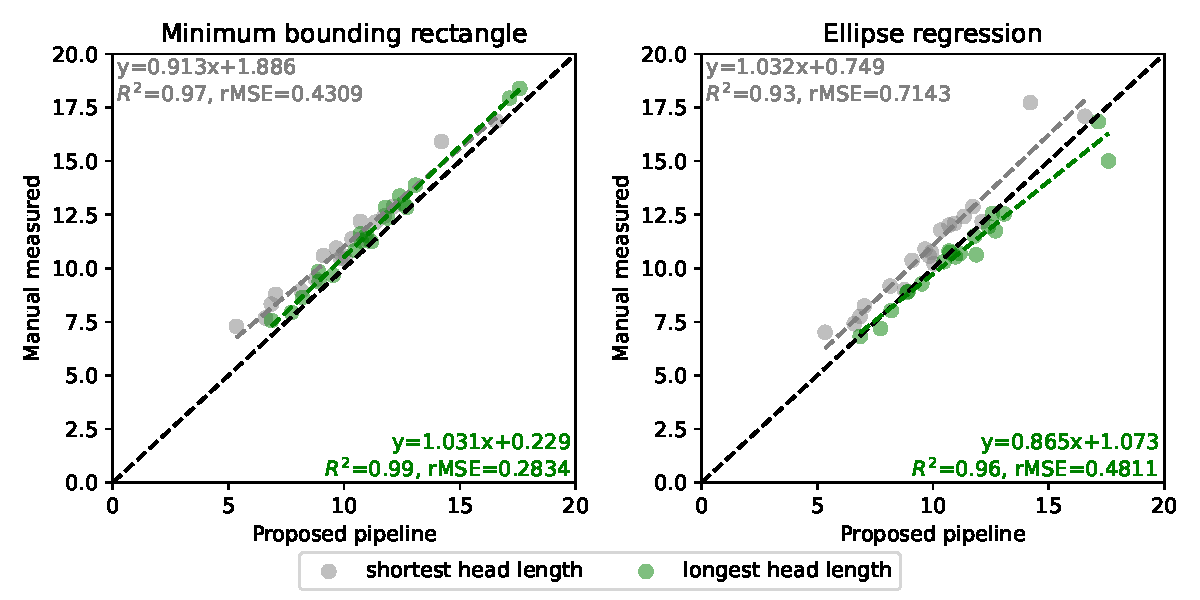
\includegraphics{figures/des/method_compare.pdf}
    }
  \end{center}
  \caption[The comparison between the proposed phenotyping pipeline and manual measurement]{
    The comparison between the proposed phenotyping pipeline and manual measurement. The shortest length and longest length of the broccoli head are compared. For the proposed pipeline, it uses two methods to estimate those lengths. One is using the length and width of the minimum bounding rectangle, the other is using the major and minor axes of the fitted ellipse.
  }
  \label{fig:des_compare}
\end{figure}

\section{Discussion}

% drawbacks: 1) only suitable for solid objects; 2) need manual flip the object, which takes over 80% of the time.


\section{Conclusion}